\documentclass[letterpaper]{article}
\usepackage[margin=1in]{geometry}
\usepackage[utf8]{inputenc}
\usepackage{textcomp}
\usepackage{amssymb}
\usepackage{natbib}
\usepackage{graphicx}
\usepackage{gensymb}
\usepackage{amsthm, amsmath, mathtools}
\usepackage[dvipsnames]{xcolor}
\usepackage{enumerate}
\usepackage{mdframed}
\usepackage[most]{tcolorbox}
\usepackage{csquotes}
% https://tex.stackexchange.com/questions/13506/how-to-continue-the-framed-text-box-on-multiple-pages

\tcbuselibrary{theorems}

\newcommand{\R}{\mathbb{R}}
\newcommand{\Z}{\mathbb{Z}}
\newcommand{\N}{\mathbb{N}}
\newcommand{\Q}{\mathbb{Q}}
\newcommand{\C}{\mathbb{C}}
\newcommand{\code}[1]{\texttt{#1}}
\newcommand{\mdiamond}{$\diamondsuit$}
\newcommand{\PowerSet}{\mathcal{P}}
\newcommand{\Mod}[1]{\ (\mathrm{mod}\ #1)}
\DeclareMathOperator{\lcm}{lcm}

%\newtheorem*{theorem}{Theorem}
%\newtheorem*{definition}{Definition}
%\newtheorem*{corollary}{Corollary}
%\newtheorem*{lemma}{Lemma}
\newtheorem*{proposition}{Proposition}


\newtcbtheorem[number within=section]{theorem}{Theorem}
{colback=green!5,colframe=green!35!black,fonttitle=\bfseries}{th}

\newtcbtheorem[number within=section]{definition}{Definition}
{colback=blue!5,colframe=blue!35!black,fonttitle=\bfseries}{def}

\newtcbtheorem[number within=section]{corollary}{Corollary}
{colback=yellow!5,colframe=yellow!35!black,fonttitle=\bfseries}{cor}

\newtcbtheorem[number within=section]{lemma}{Lemma}
{colback=red!5,colframe=red!35!black,fonttitle=\bfseries}{lem}

\newtcbtheorem[number within=section]{example}{Example}
{colback=white!5,colframe=white!35!black,fonttitle=\bfseries}{def}

\newtcbtheorem[number within=section]{note}{Important Note}{
        enhanced,
        sharp corners,
        attach boxed title to top left={
            xshift=-1mm,
            yshift=-5mm,
            yshifttext=-1mm
        },
        top=1.5em,
        colback=white,
        colframe=black,
        fonttitle=\bfseries,
        boxed title style={
            sharp corners,
            size=small,
            colback=red!75!black,
            colframe=red!75!black,
        } 
    }{impnote}
\usepackage[utf8]{inputenc}
\usepackage[english]{babel}
\usepackage{fancyhdr}
\usepackage[hidelinks]{hyperref}

\pagestyle{fancy}
\fancyhf{}
\rhead{Math 170B}
\chead{Friday, May 19, 2023}
\lhead{Lecture 21}
\rfoot{\thepage}

\setlength{\parindent}{0pt}

\begin{document}

\section{One-Variable Optimization (Section 11.1)}
Suppose we have a nonlinear function $f$ represented by the graph below, 
\begin{center}
    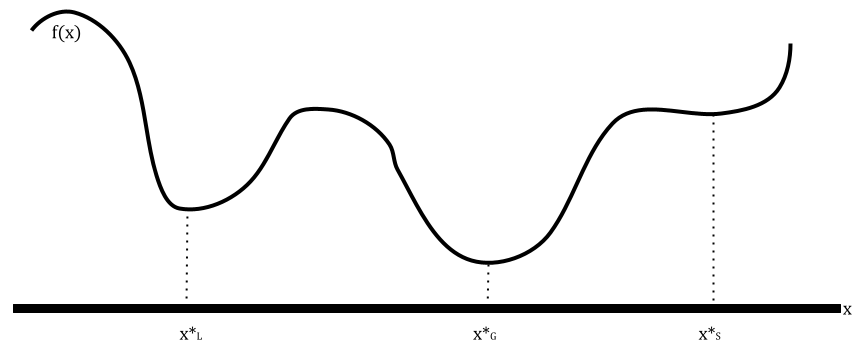
\includegraphics[scale=0.5]{../assets/1varopt_ex.png}
\end{center}
with the points 
\begin{itemize}
    \item $x^*_{L}$: the local minimum, or the smallest point of $f(x)$ in an open neighborhood around $x_{L}^*$,
    \item $x^*_{G}$: the global minimum (and also a local minimum), or the smallest minimum across the entire function, and 
    \item $x^*_{S}$: where $f$ increases or decreases on either side of $x_{S}^*$.
\end{itemize}
We're interested in the local minimum. More specifically, the goal is to find the minimum of a nonlinear function $f(x)$ (and we're fine with a local minima).

\bigskip 

1D optimization is also relevant for $\R^m$. If $F: \R^m \to \R$, then we can define a line to be $\{u + tv : t \in \R\}$, where $u, v \in \R$. Then, for a fixed $\vec{u}$ and $\vec{v}$, we can find $F(u + tv) = f(t)$. The search to find the minimum depends on what information of $f$ is available. In particular, whether we have access to $f'$ or not. 

\subsection{Illustrative Strategy (Refining Search)}
Suppose we have a bound $|f'(x)| \leq M$. The idea is that we have $x^{(k)} = hk$, with $h$ equally spaced intervals (step size) and for $k = 0, 1, 2, \hdots$. This gives us something like 
\begin{center}
    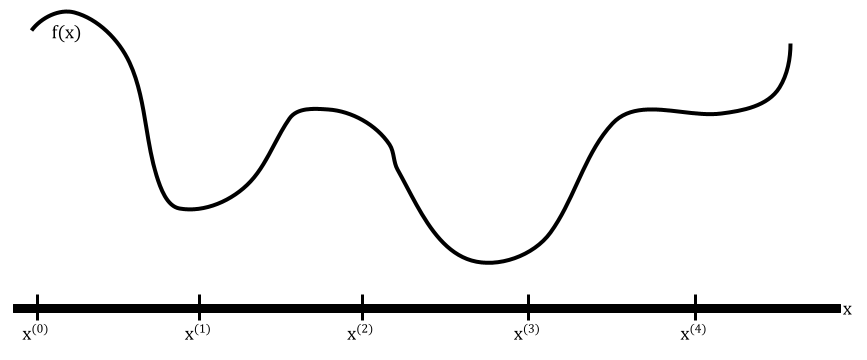
\includegraphics[scale=0.5]{../assets/1varopt_ex2.png}
\end{center}
Suppose we consider a particular interval $[a, b]$ with $a < b$. Then, 
\[f(x) \geq \min\{f(x), f(b)\} - \frac{1}{2} (b - a) M,\]
where we derived the latter part from the Mean Value Theorem. To see why this works, suppose $x$ is to the left of the midpoint between $[a, b]$. Then, 
\begin{center}
    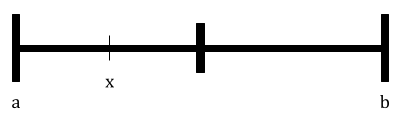
\includegraphics[scale=0.5]{../assets/interval_left.png}
\end{center}
then, by the Mean Value Theorem, \[f(x) - f(a) = f'(\xi)(x - a)\]
and \[f(x) - f(a) \geq -M\frac{1}{2}(b - a) \implies f(x) \geq f(a) - \frac{1}{2}(b - a)M.\]
In any case, if we consider all sampled points, then\footnote{We can roughly think of $\inf$ as the ``true minimum.''} 
\[\min_{k} f(x^{(k)}) \geq \inf_{x} f(x) \geq \underbrace{\min_{k} f(x^{(k)}) - \frac{1}{2}hM}_{\text{Lower Bound}}.\]
Suppose we consider the interval $[x^{(j)}, x^{(j + 1)}]$ for refinement. We then want to consider the inequality when considering the refined search:
\[\min_{k} f(x^{(k)}) + \frac{1}{2}hM \geq \min\{f(x^{(j)}), f(x^{(k + 1)})\},\]
Visually, these combined ideas would look like 
\begin{center}
    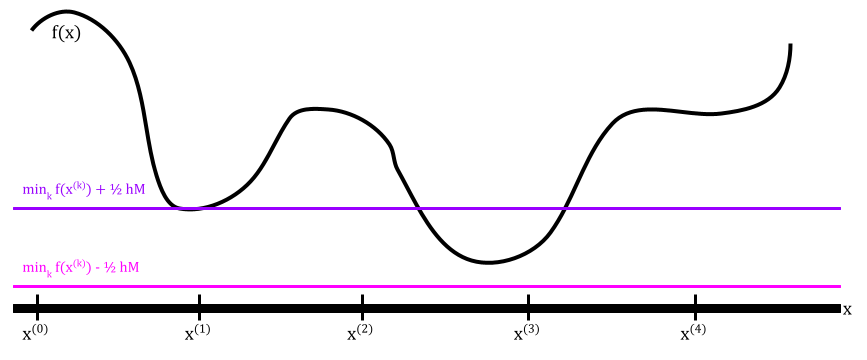
\includegraphics[scale=0.5]{../assets/1varopt_ex3.png}
\end{center}
Notice how, for example, $x^{(2)}$ and $x^{(3)}$ has a minimum. So, we would consider this interval in our refined search.

\subsection{No Derivative Strategy}
Suppose we do not have derivative information. Then, an assumption we can make is that $f$ is unimodal (i.e., one minimum). Such an example is 
\begin{center}
    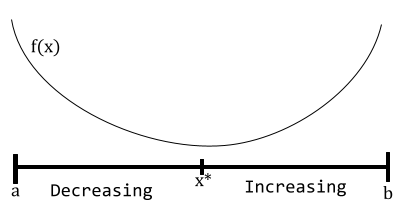
\includegraphics[scale=0.5]{../assets/no_deriv_fx.png}
\end{center}
For something like this, we might consider the \textbf{golden section search}. That is, 
\[r^2 = 1 - r\]
\[r = \frac{1}{2} \left(\sqrt{5} - 1\right) \approx 0.6180\hdots.\]
This method is similar to the bisection method. In particular, we have 
\[x = a + r(b - a) \qquad y = a + r^2 (b - a).\]
This gives us 
\begin{center}
    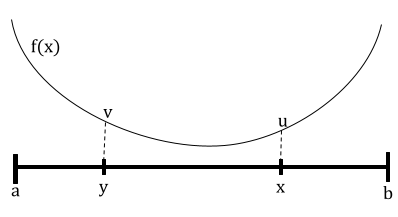
\includegraphics[scale=0.5]{../assets/no_deriv_fx1.png}
\end{center}
The search continues based on the values of $u$ and $v$. In particular, 
\begin{itemize}
    \item if $v < u$, then we want to update the right bracket.
    \item if $v \geq u$, then we want to update the left bracket.
\end{itemize}
This can be modeled into an algorithm which takes the following inputs: 
\begin{itemize}
    \item \code{a}: the first endpoint. 
    \item \code{b}: the second endpoint. 
    \item $f$: the function. 
    \item $\epsilon$: the tolerance.
    \item $M$: The maximum number of iterations.
\end{itemize}

\begin{algorithm}[H]
    \caption{Golden Section Search}
    \begin{algorithmic}[1]
        \Function{GoldenSectionSearch}{$a, b, f, \epsilon, M$}
            \State $x \gets a + r(b - a)$
            \State $y \gets a + r^2 (b - a)$
            \State $u \gets f(x)$
            \State $v \gets f(y)$
            \For{$k \gets 1$ to $M$}
                \If{$v < u$}
                    \State $b \gets x$
                    \State $x \gets y$
                    \State $u \gets v$
                    \State $y \gets a + r^2 (b - a)$
                    \State $v \gets f(y)$
                \Else 
                    \State $a \gets y$
                    \State $y \gets x$
                    \State $v \gets u$
                    \State $x \gets a + r (b - a)$
                    \State $u \gets f(x)$
                \EndIf 

                \If{$|b - a| < \epsilon$}
                    \State break
                \EndIf 
            \EndFor 
        \EndFunction
    \end{algorithmic}
\end{algorithm}

\end{document}